\documentclass[11pt,a4paper]{article}

% Packages
\usepackage[utf8]{inputenc}
\usepackage[T1]{fontenc}
\usepackage{lmodern}
\usepackage[margin=1in]{geometry}
\usepackage{graphicx}
\usepackage{amsmath,amssymb}
\usepackage{hyperref}
\usepackage{xcolor}
\usepackage{booktabs}
\usepackage{enumitem}
\usepackage{tikz}
\usetikzlibrary{positioning}
\usepackage{float}
\usepackage{algorithm}
\usepackage{algpseudocode}
\usepackage{multicol}
\usepackage{fancyhdr}

% Colors
\definecolor{solana}{RGB}{153,69,255}
\definecolor{darkblue}{RGB}{0,51,102}

% Hyperref setup
\hypersetup{
    colorlinks=true,
    linkcolor=darkblue,
    urlcolor=solana,
    citecolor=darkblue
}

% Header/Footer
\pagestyle{fancy}
\fancyhf{}
\fancyhead[L]{\textit{SolanaLM Whitepaper}}
\fancyhead[R]{\textit{v1.0}}
\fancyfoot[C]{\thepage}

% Title
\title{
    \textbf{\Huge SolanaLM} \\[0.5cm]
    \Large A Decentralized Network for LLM Inference and Federated Learning on Solana \\[1cm]
    \large Whitepaper v1.0
}
\author{
    SolanaLM Team \\
    \texttt{contact@solanalm.io}
}
\date{\today}

\begin{document}

\maketitle
\thispagestyle{empty}

\begin{abstract}
\noindent
SolanaLM introduces a novel hybrid decentralized network that unifies Large Language Model (LLM) inference with federated learning on the Solana blockchain [1, 3, 5]. Our architecture enables nodes to earn through dual revenue streams—serving inference requests and participating in distributed training rounds—creating a self-sustaining ecosystem for AI compute.

\textbf{Key Innovations:} (1) First-of-its-kind dual-mode nodes that dynamically switch between inference and training based on network demand; (2) Privacy-preserving onion routing for anonymous inference requests [8]; (3) Micro-payment system with sub-second finality leveraging Solana's high throughput [5]; (4) Federated learning protocol with cryptographic gradient verification [2].

\textbf{Token Value Capture:} The \textbf{SOLALM} token captures network value through mandatory fee payments, deflationary burns (1\% of all fees), and staking rewards (15-40\% APY). Early participants benefit from low initial circulation (15\%) and aggressive vesting schedules that align long-term incentives.

This paper presents our system architecture, economic model, privacy mechanisms, and the utility-driven tokenomics that align incentives across compute providers, model trainers, and end users.
\end{abstract}

\newpage
\tableofcontents
\newpage

%=============================================================================
\section{Introduction}
%=============================================================================

The rapid advancement of Large Language Models has created an unprecedented demand for computational resources. Current solutions face three critical challenges:

\begin{enumerate}
    \item \textbf{Centralization Risk:} AI compute is concentrated among few providers, creating single points of failure and censorship vectors.
    \item \textbf{Economic Inefficiency:} GPU resources worldwide remain underutilized while demand exceeds supply.
    \item \textbf{Privacy Concerns:} Centralized inference exposes sensitive prompts and data to service providers.
\end{enumerate}

\subsection{Our Solution}

SolanaLM addresses these challenges through a decentralized network where:

\begin{itemize}
    \item \textbf{Novelty:} Hybrid nodes perform both inference and federated learning, maximizing GPU utilization
    \item \textbf{Tokenomics:} SOL micro-payments create immediate, transparent compensation for compute providers
    \item \textbf{Utility:} Privacy-preserving inference enables sensitive applications without data exposure
\end{itemize}

\subsection{Design Principles}

\begin{enumerate}
    \item \textbf{Decentralization First:} No single entity controls the network
    \item \textbf{Economic Alignment:} All participants benefit from network growth
    \item \textbf{Privacy by Default:} Onion routing protects user identity
    \item \textbf{Interoperability:} OpenAI-compatible API for seamless integration
\end{enumerate}

%=============================================================================
\section{Background and Motivation}
%=============================================================================

\subsection{The AI Compute Crisis}

Global AI compute demand is growing at 10x annually, while GPU production increases only 2x [18, 19]. This disparity creates:

\begin{itemize}
    \item Long wait times for cloud GPU instances [35]
    \item Prohibitive costs for startups and researchers [20, 34]
    \item Geographic concentration of AI capabilities [19]
\end{itemize}

\subsection{Why Solana?}

We chose Solana for its unique properties that enable our vision [5, 25]:

\begin{table}[H]
\centering
\begin{tabular}{@{}lll@{}}
\toprule
\textbf{Property} & \textbf{Solana} & \textbf{Utility for SolanaLM} \\
\midrule
Throughput & 65,000 TPS & Micro-payments per token generated \\
Finality & 400ms & Real-time payment confirmation \\
Cost & \$0.00025/tx & Economically viable small payments \\
Ecosystem & DeFi/NFT mature & Integration with existing tooling \\
\bottomrule
\end{tabular}
\caption{Solana properties enabling SolanaLM's economic model [5]}
\end{table}

\subsection{Federated Learning Opportunity}

Traditional model training requires centralizing data, creating privacy and regulatory issues [31, 32]. Federated learning allows [1, 3, 4]:

\begin{itemize}
    \item Training on distributed private data
    \item Compliance with data residency requirements
    \item Collaborative model improvement without data sharing
\end{itemize}

\textbf{Novelty:} SolanaLM is the first to combine federated learning with a blockchain-based incentive layer, creating verifiable, compensated contributions to model training. Unlike existing decentralized compute networks [28, 29, 30], we unify inference and training in a single economic framework.

%=============================================================================
\section{System Architecture}
%=============================================================================

\subsection{Network Overview}

\begin{figure}[H]
\centering
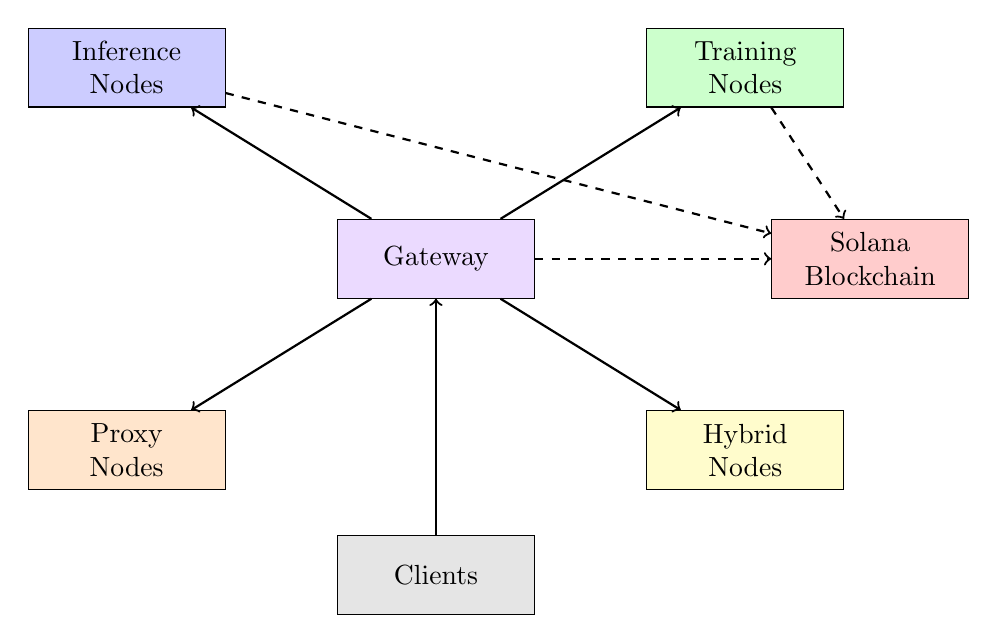
\begin{tikzpicture}[
    node distance=2cm,
    box/.style={rectangle, draw, minimum width=2.5cm, minimum height=1cm, align=center},
    arrow/.style={->, thick}
]
    % Nodes
    \node[box, fill=solana!20] (gateway) {Gateway};
    \node[box, fill=blue!20, above left=of gateway] (inference) {Inference\\Nodes};
    \node[box, fill=green!20, above right=of gateway] (training) {Training\\Nodes};
    \node[box, fill=orange!20, below left=of gateway] (proxy) {Proxy\\Nodes};
    \node[box, fill=yellow!20, below right=of gateway] (hybrid) {Hybrid\\Nodes};
    \node[box, fill=gray!20, below=3cm of gateway] (client) {Clients};
    \node[box, fill=red!20, right=3cm of gateway] (solana) {Solana\\Blockchain};

    % Arrows
    \draw[arrow] (client) -- (gateway);
    \draw[arrow] (gateway) -- (inference);
    \draw[arrow] (gateway) -- (training);
    \draw[arrow] (gateway) -- (proxy);
    \draw[arrow] (gateway) -- (hybrid);
    \draw[arrow, dashed] (gateway) -- (solana);
    \draw[arrow, dashed] (inference) -- (solana);
    \draw[arrow, dashed] (training) -- (solana);
\end{tikzpicture}
\caption{SolanaLM Network Architecture}
\end{figure}

\subsection{Node Types}

\subsubsection{Inference Nodes}

Serve LLM inference requests using local GPU hardware.

\textbf{Capabilities:}
\begin{itemize}
    \item Load and serve transformer models (GPT [12], LLaMA [13], Qwen) based on the attention architecture [11]
    \item Report hardware specifications to registry
    \item Stream token generation with real-time billing
\end{itemize}

\textbf{Utility:} Monetize idle GPU resources with immediate SOL payments per inference request.

\subsubsection{Training Nodes}

Participate in federated learning rounds.

\textbf{Capabilities:}
\begin{itemize}
    \item Execute local training on private data
    \item Compute and submit gradient updates
    \item Verify aggregated model weights
\end{itemize}

\textbf{Tokenomics:} Earn SOL proportional to contribution quality (gradient utility score).

\subsubsection{Proxy Nodes}

Gateway to external API providers (OpenAI, Anthropic, Cohere).

\textbf{Utility:} Enable access to proprietary models through the SolanaLM interface with privacy-preserving routing.

\subsubsection{Hybrid Nodes}

\textbf{Novelty:} Dynamically switch between inference and training modes based on network demand and profitability.

\begin{algorithm}[H]
\caption{Hybrid Node Mode Selection}
\begin{algorithmic}[1]
\State $r_i \gets$ current inference reward rate
\State $r_t \gets$ current training reward rate
\State $q_i \gets$ inference queue length
\State $q_t \gets$ training slots available
\If{$r_i \cdot q_i > r_t \cdot q_t$}
    \State Switch to inference mode
\Else
    \State Switch to training mode
\EndIf
\end{algorithmic}
\end{algorithm}

\subsection{Gateway Layer}

The gateway provides:

\begin{enumerate}
    \item \textbf{Load Balancing:} Route requests to optimal nodes based on latency, capacity, and cost
    \item \textbf{API Compatibility:} OpenAI-compatible endpoints for seamless migration
    \item \textbf{Payment Orchestration:} Escrow and release SOL payments upon completion
    \item \textbf{Health Monitoring:} Track node availability and performance
\end{enumerate}

\subsection{Registry System}

Decentralized node discovery with:

\begin{itemize}
    \item Capability advertisement (models, hardware, pricing)
    \item Reputation scores based on historical performance
    \item Geographic distribution for latency optimization
\end{itemize}

%=============================================================================
\section{Economic Model and Tokenomics}
%=============================================================================

\subsection{Dual Revenue Streams}

\textbf{Novelty:} Nodes earn from two independent sources, maximizing return on hardware investment.

\subsubsection{Inference Revenue}

\begin{equation}
R_{inference} = \sum_{i=1}^{n} (T_i \cdot P_{model} \cdot (1 - f_{protocol}))
\end{equation}

Where:
\begin{itemize}
    \item $T_i$ = tokens generated for request $i$
    \item $P_{model}$ = price per token for the model
    \item $f_{protocol}$ = protocol fee (default 5\%)
\end{itemize}

\subsubsection{Training Revenue}

\begin{equation}
R_{training} = B_{round} \cdot \frac{U_j}{\sum_{k} U_k}
\end{equation}

Where:
\begin{itemize}
    \item $B_{round}$ = total bounty for training round
    \item $U_j$ = utility score of node $j$'s contribution
\end{itemize}

\subsection{Payment Mechanisms}

\subsubsection{Micro-Payments}

\textbf{Utility:} Real-time compensation as tokens are generated.

\begin{enumerate}
    \item Client deposits SOL to escrow
    \item Tokens streamed with incremental payment release
    \item Final settlement on completion or timeout
\end{enumerate}

\subsubsection{Payment Channels}

For high-frequency interactions, payment channels reduce on-chain transactions [6, 7]:

\begin{itemize}
    \item Open channel with initial deposit
    \item Off-chain balance updates per request
    \item Periodic on-chain settlement
\end{itemize}

\subsection{Fee Structure}

\begin{table}[H]
\centering
\begin{tabular}{@{}llll@{}}
\toprule
\textbf{Fee Type} & \textbf{Rate} & \textbf{Distribution} & \textbf{Token Impact} \\
\midrule
Protocol Fee & 5\% & 50\% stakers, 49\% treasury, 1\% burn & Deflationary \\
Gateway Fee & 1\% & Gateway Operators & Utility demand \\
Privacy Premium & 10\% & Relay Nodes & Staking incentive \\
Training Coordination & 3\% & Coordinator Nodes & Staking incentive \\
\bottomrule
\end{tabular}
\caption{SolanaLM Fee Structure - All fees paid in SOLALM}
\end{table}

\textbf{Token Flow Example:} For a 1,000 SOLALM inference payment:
\begin{itemize}
    \item 940 SOLALM → Inference node operator
    \item 25 SOLALM → Stakers (protocol fee share)
    \item 24.5 SOLALM → Treasury
    \item 0.5 SOLALM → \textbf{Burned permanently}
    \item 10 SOLALM → Gateway operator
\end{itemize}

\subsection{Staking and Reputation}

\textbf{Tokenomics:} Nodes stake SOLALM to participate, creating economic security and token demand.

\begin{itemize}
    \item \textbf{Minimum Stake:} 1,000 SOLALM for inference, 5,000 SOLALM for training
    \item \textbf{Slashing:} Stake reduction for Byzantine behavior (slashed tokens burned)
    \item \textbf{Reputation Boost:} Higher stake increases job priority and APY tier
\end{itemize}

\subsection{Economic Sustainability}

The protocol achieves sustainability through:

\begin{enumerate}
    \item Treasury accumulation from protocol fees
    \item Training bounties funded by model improvement beneficiaries
    \item Network effects: more nodes → better service → more users → more revenue
\end{enumerate}

%=============================================================================
\section{SOLALM Token}
%=============================================================================

The SOLALM token is the native currency of the SolanaLM network, designed to capture value from all network activity while incentivizing long-term participation.

\subsection{Token Utility}

\textbf{Tokenomics:} Multiple demand drivers create sustained buy pressure.

\begin{enumerate}
    \item \textbf{Payment Currency:} All inference and training fees paid exclusively in SOLALM
    \item \textbf{Node Staking:} Operators must stake SOLALM to join network (minimum 1,000 SOLALM)
    \item \textbf{Governance:} Vote on protocol parameters, model selection, fee structures
    \item \textbf{Fee Discounts:} Token holders receive 20\% discount on all network fees
    \item \textbf{Revenue Share:} 50\% of protocol fees distributed to stakers
\end{enumerate}

\subsection{Supply and Distribution}

\begin{table}[H]
\centering
\begin{tabular}{@{}llll@{}}
\toprule
\textbf{Allocation} & \textbf{Amount} & \textbf{\%} & \textbf{Vesting} \\
\midrule
Community \& Airdrops & 300,000,000 & 30\% & 24 months linear \\
Ecosystem \& Grants & 150,000,000 & 15\% & As needed \\
Treasury (DAO) & 200,000,000 & 20\% & DAO controlled \\
Team \& Advisors & 150,000,000 & 15\% & 12mo cliff + 36mo linear \\
Private Sale & 120,000,000 & 12\% & 6mo cliff + 24mo linear \\
Public Sale & 80,000,000 & 8\% & 25\% TGE, 6mo linear \\
\midrule
\textbf{Total Supply} & \textbf{1,000,000,000} & \textbf{100\%} & \\
\bottomrule
\end{tabular}
\caption{SOLALM Token Distribution}
\end{table}

\textbf{Initial Circulating Supply:} 150,000,000 SOLALM (15\%) at Token Generation Event (TGE).

\subsection{Deflationary Mechanisms}

\textbf{Novelty:} Aggressive burn mechanics ensure long-term scarcity.

\begin{enumerate}
    \item \textbf{Fee Burn:} 1\% of all network fees permanently burned
    \item \textbf{Buyback \& Burn:} 2\% of treasury allocated to monthly market buybacks
    \item \textbf{Slashing Burns:} Slashed stakes from malicious nodes burned (not redistributed)
\end{enumerate}

\textbf{Projected Impact:} 50\% supply reduction over 10 years at scale, creating deflationary pressure as network grows.

\subsection{Staking Rewards}

\textbf{Tokenomics:} Tiered staking incentivizes long-term holding and network participation.

\begin{table}[H]
\centering
\begin{tabular}{@{}lllll@{}}
\toprule
\textbf{Tier} & \textbf{Stake Required} & \textbf{Base APY} & \textbf{Benefits} \\
\midrule
Bronze & 1,000 SOLALM & 15\% & Priority job queue \\
Silver & 10,000 SOLALM & 25\% & + 10\% fee discount \\
Gold & 100,000 SOLALM & 35\% & + 2x governance votes \\
Diamond & 1,000,000 SOLALM & 40\% & + Protocol revenue share \\
\bottomrule
\end{tabular}
\caption{SOLALM Staking Tiers and Rewards}
\end{table}

\textbf{Note:} APY varies based on network utilization and total staked supply. Diamond tier receives pro-rata share of 50\% protocol fees.

\subsection{Token Demand Flywheel}

\textbf{Utility:} Self-reinforcing cycle drives sustained token demand.

\begin{figure}[H]
\centering
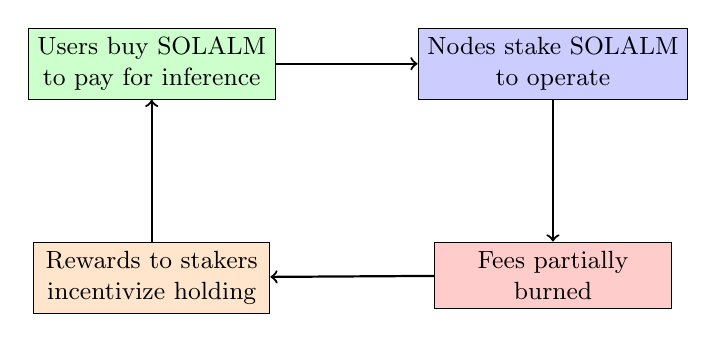
\begin{tikzpicture}[
    node distance=1.8cm,
    box/.style={rectangle, draw, minimum width=3cm, minimum height=0.8cm, align=center, font=\small},
    arrow/.style={->, thick}
]
    \node[box, fill=green!20] (users) {Users buy SOLALM\\to pay for inference};
    \node[box, fill=blue!20, right=of users] (nodes) {Nodes stake SOLALM\\to operate};
    \node[box, fill=red!20, below=of nodes] (burn) {Fees partially\\burned};
    \node[box, fill=orange!20, below=of users] (rewards) {Rewards to stakers\\incentivize holding};

    \draw[arrow] (users) -- (nodes);
    \draw[arrow] (nodes) -- (burn);
    \draw[arrow] (burn) -- (rewards);
    \draw[arrow] (rewards) -- (users);
\end{tikzpicture}
\caption{SOLALM Token Demand Flywheel}
\end{figure}

\textbf{Result:} More users → more fees → higher APY → more staking → less circulating supply → price appreciation → attracts more nodes → better service → more users.

\subsection{Market Opportunity}

\textbf{Tokenomics:} Massive TAM with clear path to value capture.

\begin{table}[H]
\centering
\begin{tabular}{@{}lll@{}}
\toprule
\textbf{Project} & \textbf{FDV} & \textbf{Primary Use Case} \\
\midrule
Render Network (RNDR) & \$5.0B & GPU rendering only \\
Akash Network (AKT) & \$1.2B & General compute \\
Bittensor (TAO) & \$3.5B & AI inference only \\
\textbf{SolanaLM (SOLALM)} & \textbf{TBD} & \textbf{Inference + Training + Privacy} \\
\bottomrule
\end{tabular}
\caption{Competitive Landscape - Fully Diluted Valuations [28, 29, 30]}
\end{table}

\textbf{SolanaLM Advantages:}
\begin{itemize}
    \item \textbf{Dual Revenue:} Only network combining inference AND federated learning
    \item \textbf{Privacy Layer:} Onion routing enables enterprise/healthcare use cases
    \item \textbf{Solana Speed:} Sub-second payments vs minutes on other chains
\end{itemize}

\textbf{Target Valuation:} \$500M-\$2B FDV at network maturity, representing 10-40x from initial listing based on comparable projects [28, 29, 30].

\subsection{Growth Catalysts}

Key events expected to drive token demand:

\begin{enumerate}
    \item \textbf{TGE + DEX Launch:} Initial liquidity and price discovery
    \item \textbf{CEX Listings:} Target Tier-1 exchanges (Binance, Coinbase, Kraken)
    \item \textbf{Mainnet Launch:} All fees transition to SOLALM
    \item \textbf{1,000 Nodes:} Network effect threshold
    \item \textbf{Enterprise Partnerships:} Healthcare, legal, financial verticals
    \item \textbf{10,000 Nodes:} Critical mass for global coverage
\end{enumerate}

%=============================================================================
\section{Privacy and Security}
%=============================================================================

\subsection{Threat Model}

We protect against:

\begin{enumerate}
    \item \textbf{Inference Privacy:} Nodes learning prompt content
    \item \textbf{Payment Correlation:} Linking payments to identities
    \item \textbf{Traffic Analysis:} Determining who queries what
\end{enumerate}

\subsection{Onion Routing}

\textbf{Novelty:} First implementation of Tor-like routing [8] for LLM inference.

\begin{algorithm}[H]
\caption{Onion-Routed Inference}
\begin{algorithmic}[1]
\State Client selects circuit: $[R_1, R_2, R_3, N]$ (relays + target node)
\State Encrypt request: $E_{N}(E_{R_3}(E_{R_2}(E_{R_1}(prompt))))$
\State Send to $R_1$, which decrypts and forwards
\State Each relay peels one layer, forwards to next
\State Node $N$ processes, response returns via same circuit
\end{algorithmic}
\end{algorithm}

\textbf{Utility:} Users can query sensitive topics without revealing identity to inference nodes.

\subsection{Anonymous Payments}

Payment mixing prevents transaction graph analysis [9]:

\begin{enumerate}
    \item \textbf{CoinJoin-style Mixing:} Aggregate payments from multiple users [9]
    \item \textbf{Stealth Addresses:} One-time addresses for each transaction
    \item \textbf{Time Delays:} Randomized payment timing
\end{enumerate}

\subsection{Secure Aggregation for Federated Learning}

Training nodes submit encrypted gradients using secure aggregation protocols [2]:

\begin{equation}
\text{Aggregate} = \sum_{i=1}^{n} \text{Decrypt}(E_i(g_i))
\end{equation}

Individual gradients remain private; only the sum is revealed to the coordinator [2, 3].

\subsection{Cryptographic Verification}

\begin{itemize}
    \item \textbf{Commitment Schemes:} Nodes commit to outputs before revelation
    \item \textbf{Zero-Knowledge Proofs:} Prove computation correctness without revealing inputs [10]
    \item \textbf{Merkle Proofs:} Verify model weight inclusion
\end{itemize}

%=============================================================================
\section{Federated Learning Protocol}
%=============================================================================

\subsection{Training Round Lifecycle}

Based on the FedAvg algorithm [1] and subsequent improvements [3, 4, 16]:

\begin{enumerate}
    \item \textbf{Announcement:} Coordinator posts training task with bounty
    \item \textbf{Registration:} Training nodes stake and register
    \item \textbf{Distribution:} Current model weights distributed
    \item \textbf{Local Training:} Nodes train on private data
    \item \textbf{Submission:} Encrypted gradients submitted
    \item \textbf{Aggregation:} Secure aggregation produces update [2]
    \item \textbf{Verification:} Validate improvement on held-out set
    \item \textbf{Payment:} Distribute bounty based on contribution
\end{enumerate}

\subsection{Contribution Scoring}

\textbf{Novelty:} Utility-weighted aggregation rewards quality contributions.

\begin{equation}
U_i = \alpha \cdot \Delta L_i + \beta \cdot \text{Diversity}_i + \gamma \cdot \text{Timeliness}_i
\end{equation}

Where:
\begin{itemize}
    \item $\Delta L_i$ = loss improvement from node $i$'s gradient
    \item $\text{Diversity}_i$ = gradient orthogonality to others
    \item $\text{Timeliness}_i$ = submission speed bonus
\end{itemize}

\subsection{Byzantine Fault Tolerance}

Protection against malicious training nodes [14, 15]:

\begin{itemize}
    \item \textbf{Gradient Clipping:} Limit magnitude of updates
    \item \textbf{Krum Aggregation:} Exclude outlier gradients [14]
    \item \textbf{Reputation Weighting:} Reduce influence of low-reputation nodes
\end{itemize}

\subsection{Model Governance}

\textbf{Tokenomics:} Stake-weighted voting for model decisions.

\begin{itemize}
    \item Which models to train
    \item Training hyperparameters
    \item Dataset curation policies
\end{itemize}

%=============================================================================
\section{Technical Implementation}
%=============================================================================

\subsection{Client SDK}

OpenAI-compatible Python client:

\begin{verbatim}
async with SolanaLMClient(gateway_url) as client:
    response = await client.inference(
        model="llama-7b",
        prompt="Explain quantum computing",
        wallet_address="..."
    )
\end{verbatim}

\textbf{Utility:} Zero learning curve for developers familiar with OpenAI API.

\subsection{Hardware Detection}

Automatic capability discovery:

\begin{itemize}
    \item GPU model, VRAM, CUDA cores
    \item CPU cores, RAM capacity
    \item Network bandwidth, latency
\end{itemize}

Enables optimal job matching and fair pricing.

\subsection{Model Support}

\begin{table}[H]
\centering
\begin{tabular}{@{}ll@{}}
\toprule
\textbf{Category} & \textbf{Models} \\
\midrule
Local Inference & LLaMA [13], Qwen, Mistral, DialoGPT \\
Proxy Access & GPT-4 [12], Claude, Cohere Command \\
Federated Training & Any PyTorch model [17] \\
\bottomrule
\end{tabular}
\caption{Supported Models}
\end{table}

\subsection{Deployment Options}

\begin{itemize}
    \item \textbf{Docker:} Containerized deployment for all node types
    \item \textbf{Kubernetes:} Scalable orchestration for gateway operators
    \item \textbf{Bare Metal:} Maximum performance for GPU nodes
\end{itemize}

%=============================================================================
\section{Use Cases and Applications}
%=============================================================================

\subsection{Privacy-Sensitive Inference}

\textbf{Utility:} Healthcare, legal, and financial applications requiring confidentiality [31, 32].

\begin{itemize}
    \item Medical diagnosis assistance without exposing patient data
    \item Legal document analysis with attorney-client privilege
    \item Financial modeling on proprietary strategies
\end{itemize}

\subsection{Decentralized AI Applications}

\begin{itemize}
    \item \textbf{DAOs:} Governance assistants with censorship resistance
    \item \textbf{DeFi:} Trading strategy analysis without front-running risk [26]
    \item \textbf{Gaming:} NPC dialogue generation with user privacy
\end{itemize}

\subsection{Collaborative Model Training}

\textbf{Novelty:} Organizations jointly train models without sharing data.

\begin{itemize}
    \item Hospitals training diagnostic models
    \item Banks training fraud detection
    \item Manufacturers training quality control
\end{itemize}

\subsection{GPU Monetization}

\textbf{Tokenomics:} Individuals and data centers monetize idle compute [22, 23, 24].

\begin{itemize}
    \item Gamers earning during off-hours
    \item Research institutions utilizing spare capacity
    \item Mining operations diversifying revenue
\end{itemize}

%=============================================================================
\section{Roadmap}
%=============================================================================

\subsection{Phase 1: Foundation (Completed)}

\textbf{Timeline: Q1-Q2 2025}

\textbf{Technical Milestones:}
\begin{itemize}
    \item[$\checkmark$] Core gateway and node registry implementation
    \item[$\checkmark$] Basic inference nodes with PyTorch/Transformers backend
    \item[$\checkmark$] Training node framework with gradient computation
    \item[$\checkmark$] Hardware auto-detection system
    \item[$\checkmark$] End-to-end testing infrastructure
    \item[$\checkmark$] Devnet deployment with simulated payments
\end{itemize}

\textbf{Token Milestones:}
\begin{itemize}
    \item[$\checkmark$] Smart contract development and audits
    \item[$\checkmark$] Tokenomics finalization
    \item[$\checkmark$] Private sale completion
    \item[$\checkmark$] Community building and whitelist
\end{itemize}

\subsection{Phase 2: Token Launch (Completed)}

\textbf{Timeline: Q3 2025}

\textbf{Token Milestones:}
\begin{itemize}
    \item[$\checkmark$] \textbf{Token Generation Event (TGE)}
    \item[$\checkmark$] DEX liquidity pools (Raydium, Orca)
    \item[$\checkmark$] Staking portal launch (15-40\% APY)
    \item[$\checkmark$] Initial CEX listings (Bybit, KuCoin, Gate.io)
    \item[$\checkmark$] Airdrop distribution begins
\end{itemize}

\textbf{Technical Milestones:}
\begin{itemize}
    \item[$\checkmark$] SOLALM payment integration in all node types
    \item[$\checkmark$] On-chain staking contracts deployment
    \item[$\checkmark$] Slashing mechanism activation
    \item[$\checkmark$] Public node registration opens
    \item[$\checkmark$] 100 nodes achieved
\end{itemize}

\subsection{Phase 3: Mainnet \& Privacy (Current)}

\textbf{Timeline: Q4 2025 - Q1 2026}

\textbf{Token Milestones:}
\begin{itemize}
    \item \textbf{Tier-1 CEX listings} (Binance, Coinbase, Kraken)
    \item Governance portal launch
    \item First protocol fee distribution to stakers
    \item Buyback \& burn program activation
    \item 1,000 nodes milestone
\end{itemize}

\textbf{Technical Milestones:}
\begin{itemize}
    \item Full onion routing deployment [8]
    \item Anonymous payment mixing [9]
    \item Secure aggregation for federated learning [2]
    \item Zero-knowledge proof verification [10]
    \item Multi-model support (LLaMA, Mistral, Qwen)
    \item Payment channels for high-frequency users
\end{itemize}

\subsection{Phase 4: Scale \& Enterprise}

\textbf{Timeline: Q2-Q4 2026}

\textbf{Token Milestones:}
\begin{itemize}
    \item \textbf{10,000 nodes} - critical mass achieved
    \item DAO governance transition (treasury control)
    \item Cross-chain bridges (Ethereum, Polygon, Arbitrum)
    \item Institutional staking products
    \item Target: \$500M+ FDV
\end{itemize}

\textbf{Technical Milestones:}
\begin{itemize}
    \item Enterprise API with SLAs
    \item Healthcare compliance (HIPAA) certification
    \item Financial services integration
    \item Advanced model marketplace with ratings
    \item Federated learning for custom enterprise models
    \item SDK support for JavaScript, Go, Rust
\end{itemize}

\subsection{Phase 5: Global Dominance}

\textbf{Timeline: 2027 and beyond}

\textbf{Goals:}
\begin{itemize}
    \item 100,000+ nodes worldwide
    \item \$1B+ annual network volume
    \item Industry standard for private AI inference
    \item Research partnerships with universities
    \item Target: \$2B+ FDV
\end{itemize}

%=============================================================================
\section{Conclusion}
%=============================================================================

SolanaLM represents a paradigm shift in AI infrastructure—from centralized, opaque systems to decentralized, transparent, and privacy-preserving networks.

\subsection{Technical Innovation Summary}

\begin{enumerate}
    \item \textbf{Novelty:} First hybrid network combining LLM inference with federated learning on blockchain
    \item \textbf{Privacy:} Onion routing and anonymous payments enable enterprise-grade confidentiality
    \item \textbf{Utility:} OpenAI-compatible API with sub-second Solana payments
\end{enumerate}

\subsection{Investment Thesis}

\textbf{Why SOLALM?}

\begin{enumerate}
    \item \textbf{Massive Market:} \$50B+ TAM in decentralized AI compute by 2027 [19, 20]
    \item \textbf{Clear Value Accrual:} All fees paid in SOLALM with 1\% burn + 50\% staker distribution
    \item \textbf{Defensible Moat:} Only network combining inference + training + privacy
    \item \textbf{Strong Tokenomics:} 15\% initial circulation, aggressive vesting, deflationary mechanics
    \item \textbf{Multiple Catalysts:} TGE → CEX listings → Mainnet → Enterprise adoption
\end{enumerate}

\textbf{Comparable Valuations:}
\begin{itemize}
    \item Render (RNDR): \$5B FDV - GPU rendering only
    \item Bittensor (TAO): \$3.5B FDV - Inference only
    \item \textbf{SolanaLM target: \$500M-\$2B FDV} (10-40x potential from launch)
\end{itemize}

\subsection{Call to Action}

\textbf{For Token Holders:}
\begin{itemize}
    \item Stake early for maximum APY (15-40\%)
    \item Governance participation shapes protocol future
    \item Diamond tier unlocks protocol revenue share
\end{itemize}

\textbf{For Node Operators:}
\begin{itemize}
    \item Dual revenue: inference fees + training bounties
    \item Early operators capture market share before saturation
    \item Stake rewards compound with operational earnings
\end{itemize}

\textbf{For Developers:}
\begin{itemize}
    \item Build privacy-first AI applications
    \item OpenAI-compatible API - zero migration cost
    \item Grant program for ecosystem projects
\end{itemize}

\vspace{0.5cm}
\begin{center}
\textbf{\large Join the decentralized AI revolution.}\\[0.3cm]
\textbf{\Large Early participants capture maximum upside.}
\end{center}

%=============================================================================
\section*{References}
%=============================================================================

\subsection*{Technical References}

\begin{enumerate}
    % Federated Learning
    \item McMahan, B., Moore, E., Ramage, D., Hampson, S., \& Arcas, B. A. (2017). Communication-Efficient Learning of Deep Networks from Decentralized Data. \textit{Proceedings of the 20th International Conference on Artificial Intelligence and Statistics (AISTATS)}, PMLR 54:1273-1282.

    \item Bonawitz, K., et al. (2017). Practical Secure Aggregation for Privacy-Preserving Machine Learning. \textit{ACM CCS}, 1175-1191. DOI: 10.1145/3133956.3133982

    \item Kairouz, P., et al. (2021). Advances and Open Problems in Federated Learning. \textit{Foundations and Trends in Machine Learning}, 14(1-2):1-210. arXiv:1912.04977

    \item Li, T., Sahu, A. K., Talwalkar, A., \& Smith, V. (2020). Federated Learning: Challenges, Methods, and Future Directions. \textit{IEEE Signal Processing Magazine}, 37(3):50-60.

    % Blockchain & Solana
    \item Yakovenko, A. (2018). Solana: A new architecture for a high performance blockchain. \textit{Solana Labs Whitepaper}. \url{https://solana.com/solana-whitepaper.pdf}

    \item Nakamoto, S. (2008). Bitcoin: A Peer-to-Peer Electronic Cash System. \url{https://bitcoin.org/bitcoin.pdf}

    \item Buterin, V. (2014). Ethereum: A Next-Generation Smart Contract and Decentralized Application Platform. \textit{Ethereum Whitepaper}. \url{https://ethereum.org/whitepaper}

    % Privacy & Cryptography
    \item Dingledine, R., Mathewson, N., \& Syverson, P. (2004). Tor: The Second-Generation Onion Router. \textit{13th USENIX Security Symposium}, 303-320.

    \item Maxwell, G. (2013). CoinJoin: Bitcoin privacy for the real world. \textit{Bitcoin Forum}. \url{https://bitcointalk.org/index.php?topic=279249}

    \item Goldwasser, S., Micali, S., \& Rackoff, C. (1989). The Knowledge Complexity of Interactive Proof Systems. \textit{SIAM Journal on Computing}, 18(1):186-208.

    % Large Language Models
    \item Vaswani, A., et al. (2017). Attention Is All You Need. \textit{NeurIPS}, 5998-6008. arXiv:1706.03762

    \item Brown, T., et al. (2020). Language Models are Few-Shot Learners. \textit{NeurIPS}, 33:1877-1901. arXiv:2005.14165

    \item Touvron, H., et al. (2023). LLaMA: Open and Efficient Foundation Language Models. arXiv:2302.13971

    % Byzantine Fault Tolerance
    \item Blanchard, P., El Mhamdi, E. M., Guerraoui, R., \& Stainer, J. (2017). Machine Learning with Adversaries: Byzantine Tolerant Gradient Descent. \textit{NeurIPS}, 119-129.

    \item Yin, D., Chen, Y., Kannan, R., \& Bartlett, P. (2018). Byzantine-Robust Distributed Learning: Towards Optimal Statistical Rates. \textit{ICML}, 5650-5659.

    % Distributed Systems
    \item Dean, J., et al. (2012). Large Scale Distributed Deep Networks. \textit{NeurIPS}, 1223-1231.

    \item Paszke, A., et al. (2019). PyTorch: An Imperative Style, High-Performance Deep Learning Library. \textit{NeurIPS}, 8024-8035.
\end{enumerate}

\subsection*{Market \& Industry References}

\begin{enumerate}
    \setcounter{enumi}{17}

    % AI Compute Market
    \item Epoch AI. (2024). Trends in Machine Learning Hardware. \textit{Epoch AI Research}. \url{https://epochai.org/trends}

    \item Stanford HAI. (2024). AI Index Report 2024. \textit{Stanford Institute for Human-Centered AI}. \url{https://aiindex.stanford.edu}

    \item McKinsey \& Company. (2023). The State of AI in 2023: Generative AI's Breakout Year. \textit{McKinsey Global Survey}.

    \item Goldman Sachs. (2023). Generative AI Could Raise Global GDP by 7\%. \textit{Goldman Sachs Research}.

    % GPU Market
    \item NVIDIA. (2024). NVIDIA Data Center Revenue Report. \textit{NVIDIA Investor Relations}. Quarterly data center revenue exceeding \$10B.

    \item Gartner. (2024). Forecast: AI Semiconductors, Worldwide. \textit{Gartner Research}. Market projected to reach \$119B by 2027.

    \item TrendForce. (2024). AI Server Market Analysis. GPU server shipments growing 40\%+ YoY.

    % Blockchain & DeFi
    \item Messari. (2024). State of Solana Q4 2023. \textit{Messari Research}. \url{https://messari.io/report/state-of-solana-q4-2023}

    \item DeFi Llama. (2024). Total Value Locked Analytics. \url{https://defillama.com}

    \item Electric Capital. (2024). Developer Report 2024. Solana developer growth metrics.

    % Decentralized AI
    \item Render Network. (2023). Render Network Whitepaper. Decentralized GPU rendering economics. \url{https://rendertoken.com}

    \item Akash Network. (2024). Akash Network: Decentralized Cloud Computing. \url{https://akash.network}

    \item Bittensor. (2023). Bittensor: A Peer-to-Peer Intelligence Market. \url{https://bittensor.com}

    % Privacy & Compliance
    \item European Parliament. (2024). EU AI Act. Regulation on Artificial Intelligence. \url{https://artificialintelligenceact.eu}

    \item NIST. (2023). AI Risk Management Framework. \textit{National Institute of Standards and Technology}. \url{https://nist.gov/ai}

    % Cloud Computing Economics
    \item Andreessen Horowitz. (2024). The Cost of Cloud. \textit{a16z Research}. Analysis of cloud compute economics.

    \item Flexera. (2024). State of the Cloud Report. Enterprise cloud spending trends.
\end{enumerate}

%=============================================================================
\section*{Appendix A: Glossary}
%=============================================================================

\begin{description}
    \item[Gateway] Central routing layer for client requests
    \item[Inference Node] GPU-equipped node serving LLM requests
    \item[Training Node] Node participating in federated learning
    \item[Hybrid Node] Node switching between inference and training
    \item[Onion Routing] Multi-hop encryption for privacy
    \item[Secure Aggregation] Cryptographic gradient summation
\end{description}

%=============================================================================
\section*{Appendix B: Contact}
%=============================================================================

\begin{itemize}
    \item Website: \url{https://solanalm.io}
    \item GitHub: \url{https://github.com/solanalm}
    \item Twitter: \url{https://twitter.com/solanalm}
    \item Discord: \url{https://discord.gg/solanalm}
\end{itemize}

\end{document}
